\documentclass[tikz,border=10pt]{standalone}
\usepackage{tikz}
\usetikzlibrary{arrows.meta}

\tikzset{
  sfgsource/.style={circle, draw=green!60!black, line width=1.2pt, minimum size=1.0cm, inner sep=0pt},
  sfgnode/.style={circle, draw=purple!70!black, line width=1.2pt, minimum size=1.0cm, inner sep=0pt},
  sfgsink/.style={circle, draw=red!70!black, line width=1.2pt, minimum size=1.0cm, inner sep=0pt},
  sfgedge/.style={->, line width=1.2pt, draw=black!80, >=Stealth},
  gain/.style={font=\small\itshape, fill=white, inner sep=1pt},
  note/.style={font=\small}
}

\begin{document}
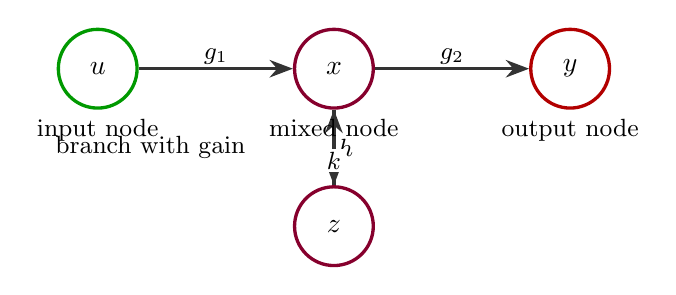
\begin{tikzpicture}
  \node[sfgsource] (u) at (0,0) {$u$};
  \node[sfgnode] (x) at (3.0,0) {$x$};
  \node[sfgsink] (y) at (6.0,0) {$y$};
  \node[sfgnode] (z) at (3.0,-2.0) {$z$};

  \draw[sfgedge] (u) -- node[gain, above] {$g_1$} (x);
  \draw[sfgedge] (x) -- node[gain, above] {$g_2$} (y);
  \draw[sfgedge] (x) -- node[gain, right] {$h$} (z);
  \draw[sfgedge] (z) -- node[gain, below] {$k$} (x);

  \node[note, anchor=north] at (u.south) {input node};
  \node[note, anchor=north] at (x.south) {mixed node};
  \node[note, anchor=north] at (y.south) {output node};
  \node[note, anchor=east] at (2.0,-1.0) {branch with gain};
\end{tikzpicture}
\end{document}
